\subsection{Filtry AI}

  Filtrowanie obrazów cyfrowych to bardzo popularny i powszechnie stosowany
  obecnie proces. Pozwala wyostrzyć niewyraźne zdjęcie, zmienić kontrast obrazu,
  czy zniwelować szumy tła. W rzeczywistości filtrowanie to nic innego, jak
  operacja matematyczna wykonywana na pikselach. Wykorzystywanie wartości wielu
  pikseli obrazu źródłowego w celu określenia wartości pojedynczego piksela w
  obrazie wynikowym. Sposób w jaki wartości te są pobierane oraz przetwarzane
  określają tak zwane maski. Przyjmują one postać macierzy kwadratowych różnych
  rozmiarów, a przechowywane w nich wartości decydują o wyniku filtracji.

  Poniższy rozdział tej pracy spróbuje udzielić odpowiedzi na pytanie, czy
  sieci neuronowe mogą sprawnie posłużyć w procesie filtrowania obrazów.
  Składa się na niego seria eksperymentów, w których specjalnie dobrane modele
  sieci spróbują odtworzyć wartości masek użytych do przygotowania danych
  treningowych, a następnie wykorzystają je do przetworzenia zupełnie nowych
  obrazów.

  Dane referencyjne składają się z zestawu obrazów przetworzonych za pomocą
  filtrów wbudowanych w bibliotekę \textit{OpenCV} takich, jak filtr Sobela, czy
  sepia.

  Wszystkie modele wytrenowane zostały w oparciu o framework TorchFrame.

  \subsubsection{Filtr Sobela}

    Jednym z podstawowych i najbardziej znanych obecnie filtrów obrazu jest
    filtr Sobela-Feldmana, który zaprezentowany został po raz pierwszy w 1968
    roku na konferencji Laboratorium Sztucznej Inteligencji uniwersytetu Stanforda
    (\textit{SAIL}). Znajduje on przede wszystkim zastosowanie w procesie wykrywania krawędzi
    na obrazach cyfrowych. Sam Irwin Sobel opisuje ten filtr następująco \cite{sobel}:

    \begin{quote}
      Motywacją w rozwijaniu tego rozwiązania było stworzenie wydajnej obliczeniowo
      estymacji gradientu, która byłaby bardziej izotropowa niż popularny wówczas operator
      "Krzyża Roberts'a".
    \end{quote}

    Operator izotropowy to, w kontekście przetwarzania obrazów, operator, którego
    działanie jest równoważne dla wszystkich kierunków na obrazie. Filtr Sobela
    wyznacza przybliżenie gradientu funkcji natężenia obrazu. Dla każdego pojedynczego
    piksela wynikiem jego działania jest wektor gradientu (lub jego długość) wskazującego kierunek wzrostu
    intensywności obrazu, wyznaczony na bazie otaczających wartości ośmiu innych pikseli.

    Na klasyczny filtr Sobela-Feldmana składają się dwie maski:

    \[G_x =
    \begin{bmatrix}
    -1 & 0 & +1 \\
    -2 & 0 & +2 \\
    -1 & 0 & +1
    \end{bmatrix}
    \]

    \[G_y =
    \begin{bmatrix}
    -1 & -2 & -1 \\
    0 & 0 & 0 \\
    +1 & +2 & +1
    \end{bmatrix}
    \]

    $G_x$ odpowiada za filtrowanie krawędzi w pionie, a $G_y$ w poziomie. Obie maski
    mogą być stosowane oddzielnie. Sam proces filtrowania bazuje na konwolucji
    opisanej w ramach sieci splotowych w rozdziale \ref{sieci_splotowe}, polegającej na
    równomiernym przesuwaniu stosowanych filtrów wzdłuż analizowanego obrazu, przy
    jednoczesnym wykonywaniu zdefiniowanych w nich obliczeń w każdym punkcie. Można
    w tym miejscu dostrzec spore podobieństwo pomiędzy klasycznymi maskami i ich zastosowaniem,
    a neuronami wchodzącymi w skład warstw konwolucyjnych sztucznych sieci splotowych. Nie bez powodu
    neurony te nazywane są filtrami.

    W przeprowadzonych doświadczeniach zastosowany został filtr Sobela z
    maską $G_x$. Zbiór uczący wykorzystywany w procesie treningu sieci składał się
    z różnorodnych obrazów dobieranych w sposób losowy. Przykładowe zdjęcia wchodzące
    w skład tego zbioru przedstawia Rysunek \ref{fig:dataset_filters}.

    \begin{figure}[H]
      \centering
      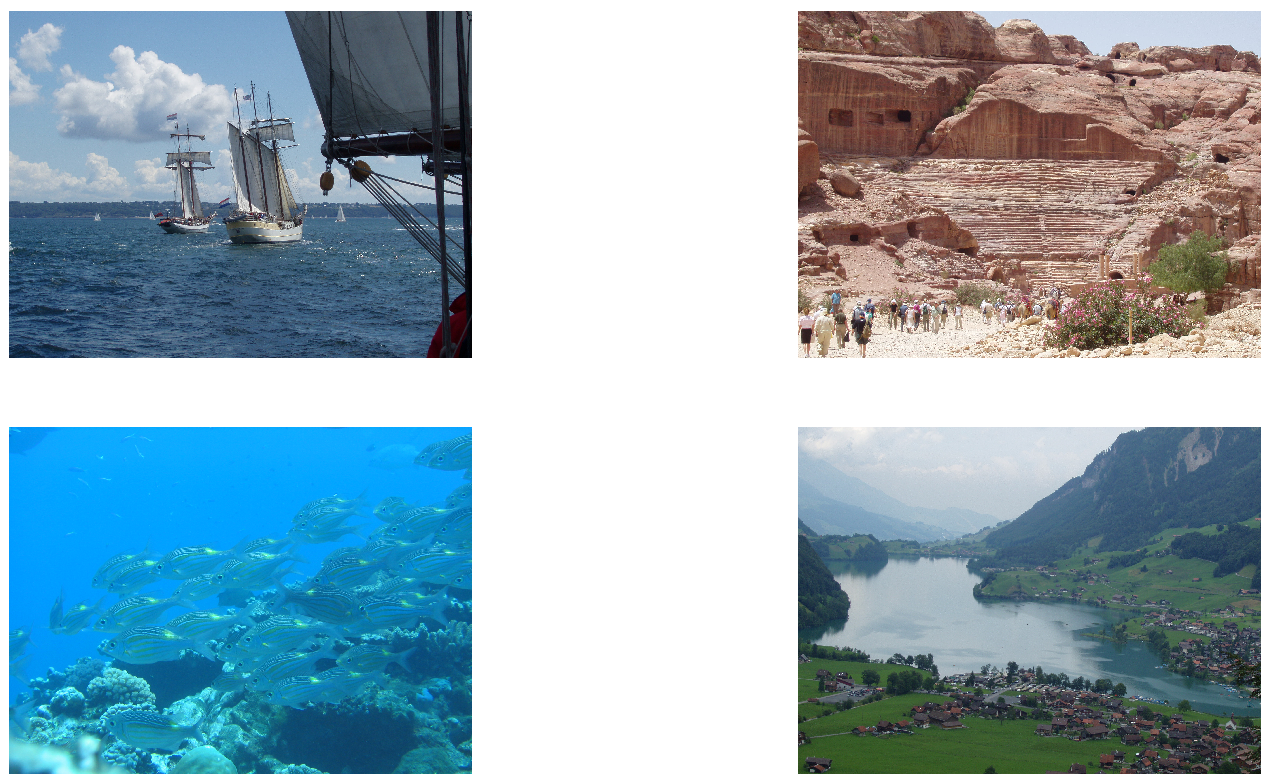
\includegraphics[width=6in]{dataset_filters}
      \caption[Przykładowe obrazy ze zbioru treningowego - źródło: Praca własna]{Przykładowe obrazy ze zbioru treningowego}
      \label{fig:dataset_filters}
    \end{figure}

    Aby mogły właściwie pełnić swoją rolę obrazy treningowe zostały w pierwszej kolejności
    poddane odpowiedniemu przetworzeniu wstępnemu. W ramach tego procesu rozmiar każdego zdjęcia
    zmniejszony został do wymiarów $256x256$ pikseli, a wartości kolorów ograniczone
    do zakresy $<-1, 1>$ w celu usprawnienia obliczeń wykonywanych przez sieć m.in.
    poprzez zapobieganie zjawisku eksplodującego gradientu. Dodatkowo w przypadku tego
    filtru zastosowana została konwersja obrazów do formatu czarno-białego, co pozwoliło
    wyodrębnić pojedynczy kanał kolorystyczny z oryginałów. Tak przetworzony zbiór uczący
    podawany był na wejście sieci neuronowej, a rezultaty jej pracy porównywane
    z obrazami na które dodatkowo nałożony został filtr Sobela za pomocą biblioteki
    \textit{OpenCV}.

    Sam model sieci składa się w tym przypadku z pojedynczego neuronu w warstwie
    konwolucyjnej, filtrującego obraz za pomocą macierzy kwadratowej stopnia
    trzeciego. Odzwierciedla to oryginalną macierz filtracji $G_x$ w stosunku jeden
    do jednego, ponieważ każda z dziewięciu wag sieci odpowiada jednemu polu w tej
    macierzy.

     

  \subsubsection{Sepia}


  \subsubsection{Filtr górnoprzepustowy}
